\documentclass{article}

\usepackage{ctex}
\usepackage{graphicx}
\graphicspath{{pic}}
\usepackage{amsmath}

\title{Week 3: git}
\author{Mayrain}
\date{\today}

\begin{document}

\maketitle

\section{Git}

\subsection{What is git}

\noindent
一个分布式的版本控制系统。分布式代表不需要联网,版本控制代表可以回溯文件修改历史。\\
有趣的部分:git是自托管的,也就是说git他自己的代码就是放在git仓库里的。现在你甚至可以在github上看到git的源代码。实现是用1000多行代码完成的。\\
git自带的git bash是一个命令行工具,可以用来操作git。他也很有用。\\

\subsection{How git works}

\noindent
\begin{align}
    working\quad directory & -> staging\quad area & ->  git  repository \notag \\
                           & add                  & commit \notag
\end{align}
他妈的这一段真丑啊我去,我得搞明白为什么排版会变成这样,但是不是现在。\\
push: 本地仓库 -> 远程仓库\\
pull: 远程仓库 -> 本地仓库\\
在这里课程讲的很简单,最好参见网络教程。\\
\\
利用git init folder可以新建一个文件夹并将其转化为git仓库。\\
git文件有三种状态:
\begin{itemize}
    \item untracked: 未跟踪
    \item modified: 已修改
    \item staged: 已暂存
    \item ignored: 已忽略
\end{itemize}
这里的ignored是指git不会跟踪这个文件,也就是说这个文件不会出现在git status的结果中。他被存储在gitignore文件。一般我们都在这里加一些规则。\\
github/gitignore: 这里有很多gitignore的规则,可以直接复制。\\
\\
commit message standards:\\
angular/angular:CONTRIBUTING.md\\
\\
作者的话:\\
老天,连git的commit的message都在github上有标准化的规定,不得不说这就是程序员的思维:机械而规范。让我想起了github上有名的“how to ask questions wisely”系列。很有意思。\\
\subsubsection{ADDITION:Commit Message Format}
*It is totally copy of angular/CONTRIBUTING.md.\\
\\
<header>\\
\\
Format: -> <Commit Type>(<Commit Scope>): <Short summary>\\
\\
Commit Type:\\
build: Changes that affect the build system or external dependencies (example scopes: gulp, broccoli, npm)\\
修改项目构建系统的代码或者外部依赖的改动,例如构建脚本,Dockerfile,package.json,webpack配置等等\\
ci: Changes to our CI configuration files and scripts (examples: CircleCi, SauceLabs)\\
修改项目继续集成流程的提交,例如Travis,Jenkins,GitLab CI,BrowserStack,SauceLabs等等\\
docs: Documentation only changes\\
仅仅修改了文档,比如README,CHANGELOG,CONTRIBUTE等等\\
feat: A new feature\\
新功能\\
fix: A bug fix\\
修复bug\\
perf: A code change that improves performance\\
提升性能的代码改动\\
refactor: A code change that neither fixes a bug nor adds a feature\\
代码重构\\
test: Adding missing tests or correcting existing tests\\
测试用例的变动\\
\\
Commit Scope:\\
indicate the place of the commit change.Should be the name of the npm package affected.Better to see this:\\
https://github.com/angular/angular/blob/main/CONTRIBUTING.md\\
\\
<Blank Line>\\
\\
<content>\\
\\
<Blank Line>\\
\\
<footer>\\
\\
\subsubsection{Version Name change rules}
version a.b.c[-d]\\
a: major version(主版本号,大改,不兼容的API修改。0表示开发阶段,不保证完整性)\\
b: minor version(次版本号,添加新功能,保持兼容)\\
c: patch version(修订号,兼容更改以及修正不正确的行为)\\
d: pre-release version(预发布版本号,代表这个程序是预发布的,实际上只是尝鲜版。顺序是alpha(内测), beta(公测), rc.1, rc.2, rc开头的都是预发布。)\\
\\
\subsection{Git Branch}
Branch,也就是分支,是相当于一个岔路指向标。在git中,我们可以创建分支,然后在分支上进行修改,最后将分支合并到主分支上。\\
如果我们在某个历史版本上做出一个修改,而不添加branch的话,那么当我们想要回到修改的版本时,就会发现我们的指针依然在master这个大branch上移动,而这个修改的版本,除非你记住了他的commit id,否则就无法回到这个版本了。(因为没有路标通向他,所以当到达分叉路口时系统会自动以为只有一条路,也就是master分支)\\
有两种创建分支的方法:\\
\begin{itemize}
    \item git branch <branch name>(基于当前的header,也就是分岔路口)
    \item git branch <branch name> <branch id>(基于当前所在分支的id提交,也就是根据这条路提交)
\end{itemize}
\section{github}
\noindent
GithubCLI是一个命令行程序,通过这个程序可以使用命令行操控github。\\
现在很多没能注意的就是,github的commit需要用签名去验证。在git中会出现一个verfied的图标,证明我使用我的私钥签名,并可以用公钥去验证。对比图如下:\\
\begin{figure}[h]
    \centering
    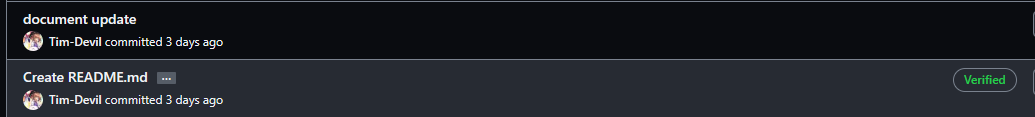
\includegraphics[width=\textwidth]{pic1_verfied.png}\\
\end{figure}

\end{document}